%卒論中間審査用研究概要テンプレート ver. 1.1

\documentclass[uplatex,twocolumn]{jsarticle}
\usepackage[top=22mm,bottom=22mm,left=20mm,right=20mm]{geometry}
\setlength{\columnsep}{15mm}
\usepackage[T1]{fontenc}
\usepackage{txfonts}
\usepackage{wrapfig}
\usepackage[expert,deluxe]{otf}
\usepackage[dvipdfmx,hiresbb]{graphicx}
\usepackage[dvipdfmx]{hyperref}
\usepackage{pxjahyper}
\usepackage{secdot}

\makeatletter
\renewcommand{\section}{%
  \@startsection{section}{1}{\z@}%
  {0.6\Cvs}{0.4\Cvs}%
  {\normalfont\normalsize\raggedright}}
\renewcommand{\subsection}{\@startsection{subsection}{2}{\z@}%
  {\z@}{\z@}%
  {\normalfont\normalsize}}
\renewcommand{\subsubsection}{\@startsection{subsubsection}{3}{\z@}%
  {\z@}{\z@}%
  {\normalfont\normalsize}}
\makeatother
%ここから上を編集する必要はない.





%タイトルと学生番号,名前だけ編集すること
\title{\vspace{-5mm}\fontsize{14pt}{0pt}\selectfont オンラインショッピングサイト利用者による商品に対するレビューの動向調査}
\author{\normalsize プロジェクトマネジメントコース・ソフトウェア開発管理グループ 矢吹研究室 1242042 齋藤 勇也}
\date{}
\pagestyle{empty}
\begin{document}
\fontsize{10.5pt}{\baselineskip}\selectfont
\maketitle





%以下が本文
\section{研究の背景}




インターネットを利用した電子商取引は1994年に米国のピザハットが行ったのが最初であるといわれている\cite{sugasaka2003}.
今まで,商品の購入方法は商品の下に足を運ぶ必要があった.この時点では商品を購入した人物は直接顔を合わせた相手にのみにしかレビューを語ることが出来ない状態である.

さらに,全ての商取引における電子取引の割合が2014年時点で3.7%となり,2008年の1.8%比べ 倍近く上昇していることから,仮想空間でも商品の売買が行いやすい環境である\cite{keizai2014}.仮想空間での商品の売買頻度が増加した1994年以降は,相対的に電子商取引であるオンラインショッピングのレビューが重要視されている.


レビューが実装されている有名なオンラインショッピングサイトでは,利用者は商品についてのレビューを記入することや,商品に得点を付けることが可能である.例えば,Amazonのレビューでは\label{customerReview}[図1]おすすめ度と称して平均値しか表示していない.実際に商品とは一切関係のないレビューや明らかに商品に対して理解が足りないレビューがあり,それらのような本来加えるべきでないレビューも多々存在する.

そこで,レビューの表示が平均評価のでは商品の判断材料としての指標が少ない.そこで平均値以上に信頼できる方法を探そうと考えた\cite{hattori2011} \cite{yamazawa2006}.


\begin{figure}[htbp]
\begin{flushleft} %左寄せ
\vspace*{-\intextsep}
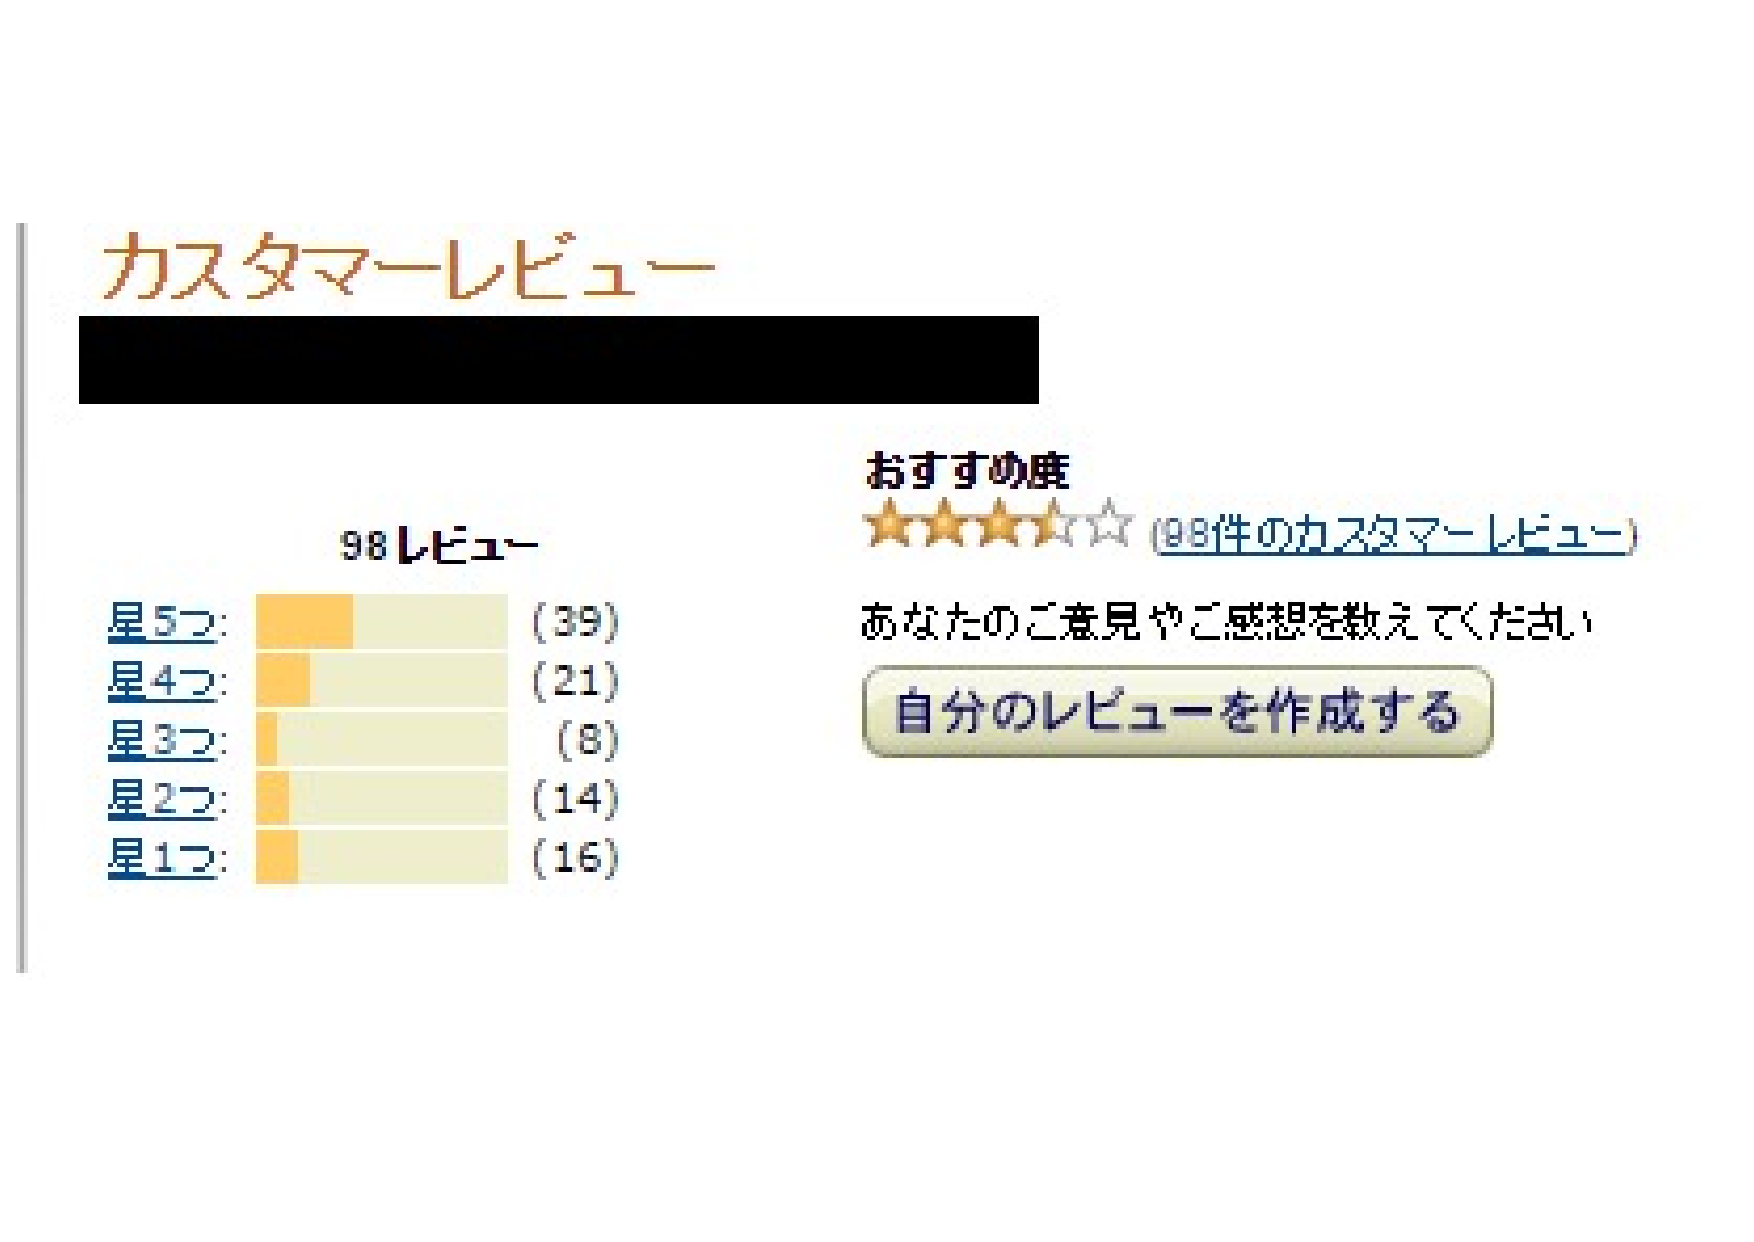
\includegraphics[width=4cm,clip]{customerReview.pdf}
\caption{Amazonでのレビューの一例}
\label{customerReview}
\end{flushleft}
\end{figure}
%\bigskip


\section{目的}

Amazonのレビューは平均値を表示している\label{customerReview} [図1].
他の指標を加え判断材料を増やすことで,平均値以上の信頼できるレビューを作る.

\section{研究方法}

レビューが嘘偽り,無関係の情報であるとしても平均値ではその状態のまま反映してしまう.そのためレビューの信頼性が低いと判断した.
なので,集合知を利用し,各レビューごとにどの程度信頼できるかを評価し信頼性をあげることを目標とする.

方法の一つとして読んだレビューが参考になるかを判断するシステムを利用し,各レビューの判断指標とすることがあげられる.
このようにそのレビューをどの程度信用できるかを判断できる項目を付け足していくことで信頼度をあげる.


\section{成果物のイメージ}

レビューを評価する項目を増やし,それらを照らし合わせ分析することでレビューの信頼度を上げる.

\section{進捗状況}

Amazonで購入した人物を絞り込むことが可能だと判明したので購入した,していない人物を分類分けすることで新たな評価基準を作り出している.

\section{今後の計画}


更なる分類分けを行い,項目を増やしていく.
同時に,対象の項目にあわせた分析方法を進める.

\bibliographystyle{junsrt}
\bibliography{biblio}%「biblio.bib」というファイルが必要.

\end{document}
